\chapter{Tree-structure segmentation for logistic regression} \label{chap6}

\epigraph{.}{.}

\minitoc


\textit{Nota Bene :} Ce chapitre s'inspire fortement ... \textcolor{red}{à adapter au moment de l'envoi du manuscrit}

\bigskip

\selectlanguage{english}

In Chapter~\ref{chap1}, and parallel to quantization, it was argued in Section~\ref{subsec:segmentation} that, what is referred to as ``segmentation'' in the \textit{Credit Scoring} industry, could also be a straightforward solution to deal with missing values and outliers. The more theoretical justification of quantization, sketched in Section~\ref{sec:bias_variance_quant}, was to achieve a good bias-variance tradeoff of the predictive task. This goal was embedded in the proposed quantization algorithm. Here again, the resulting segmentation and scorecards therein can be viewed as a single model for the whole population. In the next Section, we give some industrial context to the problem which is followed in Section~\ref{sec:literature} by a literature review. Section~\ref{sec:model_selec_tree} reinterprets this problem, as promised, as a model selection problem for which a specific approach is designed in subsequent Sections.


\section{Introduction}

\subsection{Context}

As was emphasized in all previous Chapters, \gls{lr} is the building block of a scorecard predicting the creditworthiness of an applicant and partly automating the acceptance / rejection mechanism. However, estimating \gls{lr} coefficients means that training data $(\glssymbol{bbx},\glssymbol{bby})$ is available. This is not the case when a new product, \textit{e.g.}\ smartphone leasing, is added to the acceptance system. On a practical note, some other previously learnt scorecard may not be applicable on this new market because the same information is not asked to applicants, \textit{e.g.}\ marital status, because given the low amounts at stake, it was decided to collect the fewest data possible, to make the process as simple and quick as possible. On a more theoretical note, it is probable that applicants to smartphone leasing are not stemming from the same data generating mechanism $p(\glssymbol{bX},Y)$ as the .



En matières de crédit à la consommation, les instituts financiers cherchent à automatiser la d´ecision de financement tout en ne sélectionnant que les clients susceptibles de rembourser ledit crédit. Depuis une quarantaine d’années, le Credit Scoring consiste à construire des modèles de classification supervisée $p_{\glssymbol{bth}}$ à partir des données demandées au clients $\glssymbol{bx} = (x_j)_1^d$ et de l’observation du remboursement des clients passés $y \in \{0, 1\}$. Historiquement, des scores différents sont développés sur des marchés (\textit{e.g.}\ grande distribution, électroménager, \dots) et/ou des produits (e.g. renouvelable, amortissable, \dots) et/ou des partenaires et/ou des profils clients différents dans l’esprit de la figure~\ref{fig:arbre}. Ce découpage est historique et relève d’un \textit{a priori}. On cherche ici à rationnaliser cette pratique en considérant le cluster d’appartenance du client comme un paramètre à optimiser. Si l’on note $K$ le nombre de scores à construire (inconnu) et $c = 1..K$ chaque score, correspondant à un cluster de clients, le mélange de régressions logistiques s’écrit : $p(y|x) = \sum_{c=1}^K p_{\glssymbol{bth}_c}(y|x, c)p(c|x)$, où l’on restreint $p(c|x)$ à prendre la forme de la figure~\ref{fig:arbre}, de telle sorte que le mélange n’est pas “flou” comme pour un modèle de mélange classique où la contribution de chaque classe est pondérée par sa probabilité. La
difficulté d’une approche directe réside dans cette contrainte discrète.


\tikzstyle{level 1}=[level distance=2cm, sibling distance=7cm]
\tikzstyle{level 2}=[level distance=2cm, sibling distance=4cm]
\tikzstyle{level 3}=[level distance=2cm, sibling distance=3cm]

\begin{figure}
\resizebox{\textwidth}{!}{
\centering
\begin{tikzpicture}
  [
    sibling distance        = 15em,
    level distance          = 5em,
    edge from parent/.style = {draw, -latex},
    every node/.style       = {font=\footnotesize},
    sloped
  ]
  \node [root] {\textcolor{black}{Applicants}}
    child { node [dummy] {}
      child { node [dummy] {}
        child { node [env] {\textcolor{black}{$p_{\glssymbol{bth}_1}(y|\q^1(\glssymbol{bx})))$}}
          edge from parent node [below] {Renters} }
        child { node [env] {\textcolor{black}{$p_{\glssymbol{bth}_2}(y|\q^2(\glssymbol{bx}))$}}
          edge from parent node [above] {Salaried} }
        child { node [env] {\textcolor{black}{$p_{\glssymbol{bth}_3}(y|\q^3(\glssymbol{bx}))$}}
                edge from parent node [above] {Others} }
        edge from parent node [above] {Revolving} }
      child { node [env] {\textcolor{black}{$p_{\glssymbol{bth}_4}(y|\q^4(\glssymbol{bx}))$}}
              edge from parent node [above, align=center]
                {Standard loan} }
              edge from parent node [above] {Home Appliances} }
    child { node [dummy] {}
      child { node [dummy] {}
        child { node [env] {\textcolor{black}{$p_{\glssymbol{bth}_5}(y|\q^5(\glssymbol{bx}))$}}
          edge from parent node [above] {Leasing} }
        child { node [env] {\textcolor{black}{$p_{\glssymbol{bth}_6}(y|\q^6(\glssymbol{bx}))$}}
                edge from parent node [above] {Standard loan} }
        edge from parent node [above] {Fiat} }
      child { node [env] {\textcolor{black}{$p_{\glssymbol{bth}_7}(y|\q^7(\glssymbol{bx}))$}}
              edge from parent node [above, align=center]
                {Kawasaki} }
              edge from parent node [above] {Automobile} };
\end{tikzpicture}
}
\caption{Simplified cartography of the application scorecards.}
\label{fig:arbre}
\end{figure}




\subsection{In-house \textit{ad hoc} practice}

Additionally to 



\subsection{These practices can fail}



\begin{figure}
\centering
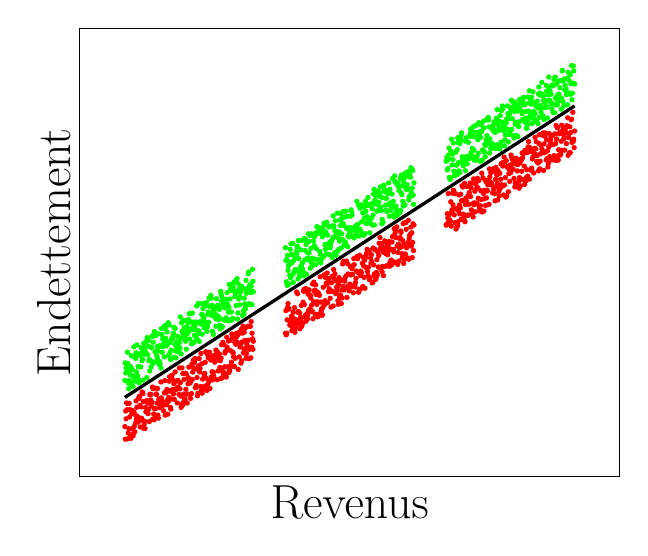
\begin{tikzpicture}


\begin{axis}[xtick=\empty, ytick=\empty, xlabel={\LARGE Revenus}, ylabel={\LARGE Endettement}]
\myGlobalTransformation{0}{0};

% pauvres
\addplot [red, only marks, mark=*, samples=300, mark size=0.75,domain=-3:1]{rand+x};
\addplot [green, only marks, mark=*, samples=300, mark size=0.75,domain=-3:1]{rand+x+2.5};

%moyens
\addplot [red, only marks, mark=*, samples=300, mark size=0.75,domain=2:6]{rand+x};
\addplot [green, only marks, mark=*, samples=300, mark size=0.75,domain=2:6]{rand+x+2.5};

%riches
\addplot [red, only marks, mark=*, samples=300, mark size=0.75,domain=7:11]{rand+x};
\addplot [green, only marks, mark=*, samples=300, mark size=0.75,domain=7:11]{rand+x+2.5};

%frontière
\addplot [black, very thick, domain=-3:11] {x+1.25};
\end{axis}


\end{tikzpicture}
\caption{\label{fig:xdiff} blabla}
\end{figure}












\begin{figure}
\centering
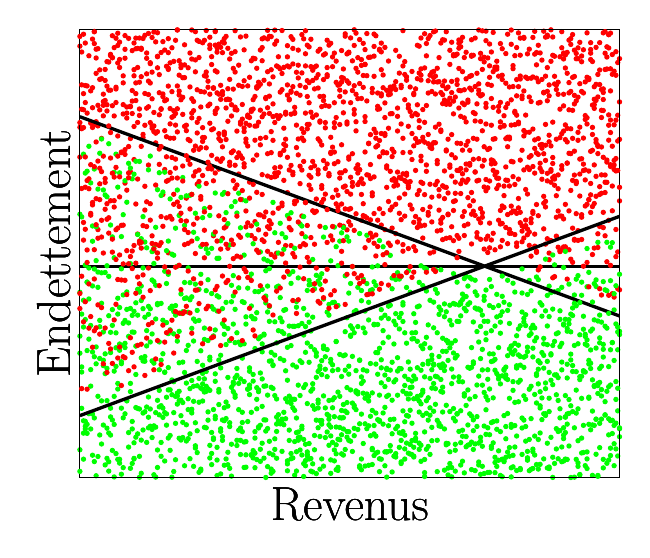
\begin{tikzpicture}


\begin{axis}[xtick=\empty, ytick=\empty, xlabel={\LARGE Revenus}, ylabel={\LARGE Endettement},domain=-3:1, enlargelimits=false,ymin=-3,ymax=6]
\myGlobalTransformationbis{0}{0};

% techniciens
\addplot [green, only marks, mark=*, samples=300, mark size=0.75,domain=-3:1]{rand};
\addplot [green, only marks, mark=*, samples=300, mark size=0.75,domain=-3:1]{rand-2};
\addplot [green, only marks, mark=*, samples=300, mark size=0.75,domain=-3:1]{rand-4};
\addplot [red, only marks, mark=*, samples=300, mark size=0.75,domain=-3:1]{rand+2.5};
\addplot [red, only marks, mark=*, samples=300, mark size=0.75,domain=-3:1]{rand+4.5};
\addplot [red, only marks, mark=*, samples=300, mark size=0.75,domain=-3:1]{rand+6.5};

%frontière
\addplot [black, very thick, domain=-3:1] {1.25};
\end{axis}





\begin{axis}[xtick=\empty, ytick=\empty, xlabel={\LARGE Revenus}, ylabel={\LARGE Endettement},domain=-3:1, enlargelimits=false,ymin=-3,ymax=6]
\myGlobalTransformationbis{0}{3};

% cadres
\addplot [green, only marks, mark=*, samples=300, mark size=0.75,domain=-3:1]{rand-x};
\addplot [green, only marks, mark=*, samples=300, mark size=0.75,domain=-3:1]{rand-x-2};
\addplot [green, only marks, mark=*, samples=300, mark size=0.75,domain=-3:1]{rand-x-4};
\addplot [red, only marks, mark=*, samples=300, mark size=0.75,domain=-3:1]{rand-x+2.5};
\addplot [red, only marks, mark=*, samples=300, mark size=0.75,domain=-3:1]{rand-x+4.5};
\addplot [red, only marks, mark=*, samples=300, mark size=0.75,domain=-3:1]{rand-x+6.5};

%frontière
\addplot [black, very thick, domain=-3:1] {-x+1.25};
\end{axis}



\begin{axis}[xtick=\empty, ytick=\empty, xlabel={\LARGE Revenus}, ylabel={\LARGE Endettement},domain=-3:1, enlargelimits=false,ymin=-3,ymax=6]
\myGlobalTransformationbis{0}{6};

% libérales
\addplot [green, only marks, mark=*, samples=300, mark size=0.75,domain=-3:1]{rand+x};
\addplot [green, only marks, mark=*, samples=300, mark size=0.75,domain=-3:1]{rand+x-2};
\addplot [green, only marks, mark=*, samples=300, mark size=0.75,domain=-3:1]{rand+x-4};
\addplot [red, only marks, mark=*, samples=300, mark size=0.75,domain=-3:1]{rand+x+2.5};
\addplot [red, only marks, mark=*, samples=300, mark size=0.75,domain=-3:1]{rand+x+4.5};
\addplot [red, only marks, mark=*, samples=300, mark size=0.75,domain=-3:1]{rand+x+6.5};
\addplot [red, only marks, mark=*, samples=300, mark size=0.75,domain=-3:1]{rand+x+8.5};

%frontière
\addplot [black, very thick, domain=-3:1] {x+1.25};
\end{axis}



\end{tikzpicture}
\caption{\label{fig:ydiff} bla}
\end{figure}








\section{Litterature review} \label{sec:literature}


\subsection{Clustering methods}


\subsection{Direct approaches: logistic regression trees}



\section{Logistic regression trees as a combinatorial model selection problem} \label{sec:model_selec_tree}


\subsection{Cardinality example}


\subsection{Logistic regression tree selection}



\section{A mixture and latent feature-based relaxation}




\section{A stochastic estimation strategy}


\section{Numerical experiments}


\subsection{Empirical consistency on simulated data}

\subsection{Benchmark on \textit{Credit Scoring} data}




\bigskip

Ce chapitre.


\printbibliography[heading=subbibliography, title=References of Chapter 5]

